\section{РУКОВОДСТВО ПО ЗАПУСКУ}
\label{sec:bootstrap}

Спроектированная система может быть портирована на любую плату с
микросхемой FPGA седьмой серии от компании Xilinx. На плате
должна присутствовать минимально необходимые компоненты:
\begin{itemize}
  \item микросхема 7 поколения компании Xilinx;
  \item микросхема SDRAM DDR;
  \item контроллер и разъём HDMI;
  \item выводы общего назначения.
\end{itemize}

Для подключения камеры используются выводы общего назначения,
прошивка бистрима осуществляется по JTAG, в основном
подключенный к конвертеру USB.

Сборка проекта осуществляется в системе автоматического проектирования
\en{Vivado}, более ранняя САПР \en{ISE Design Suite} не поддерживает
седьмое поколение микросхем FPGA.

Рассмотрим настройку, сборку и загрузку проекта на отладочную плату
поэтапно.

\subsection{Настройка проекта}
\label{sec:bootstrap:configuration}

После запуска Vivado появляется главный экран, на котором необходимо выбрать
окно текущего проекта. Для импортирования проекта необходимо:
\begin{itemize}
  \item скачать исходный код проекта в виде набора HDL модулей, IP-ядер и TCL скриптов;
  \item переместить исходный код проекта в рабочую директорию;
  \item перейти в папку с проектам при помощи команды \texttt{cd} в TCL консоли Vivado;
  \item ввести команду \texttt{source project\_name.tcl}.
\end{itemize}

Иллюстрация последних двух действий приведена на рисунке~\ref{fig:bootstrap:configuration:source}

\begin{center}
  \centering
  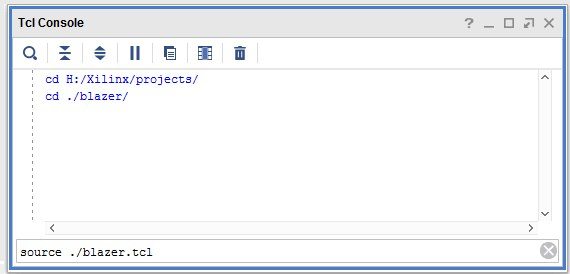
\includegraphics[scale=0.5]{source_project.jpg}
  \captionof{figure}{Развёртывание проекта в среде Vivado}
  \label{fig:bootstrap:configuration:source}
\end{center}

При использовании иной отладочной платы или камеры необходимо изменить отображение внутренней
логики на выводы микросхемы. Перепланировка выводов микросхемы осуществляется либо в специальном
разделе \en{I/O Planning} в разделе меню \en{Tools}, либо задать соотвествие в \en{constraints}
файле проекта. Дерево выбора \en{constraints} файла представлено на рисунке~\ref{fig:bootstrap:configuration:constraints_tree}

\begin{center}
  \centering
  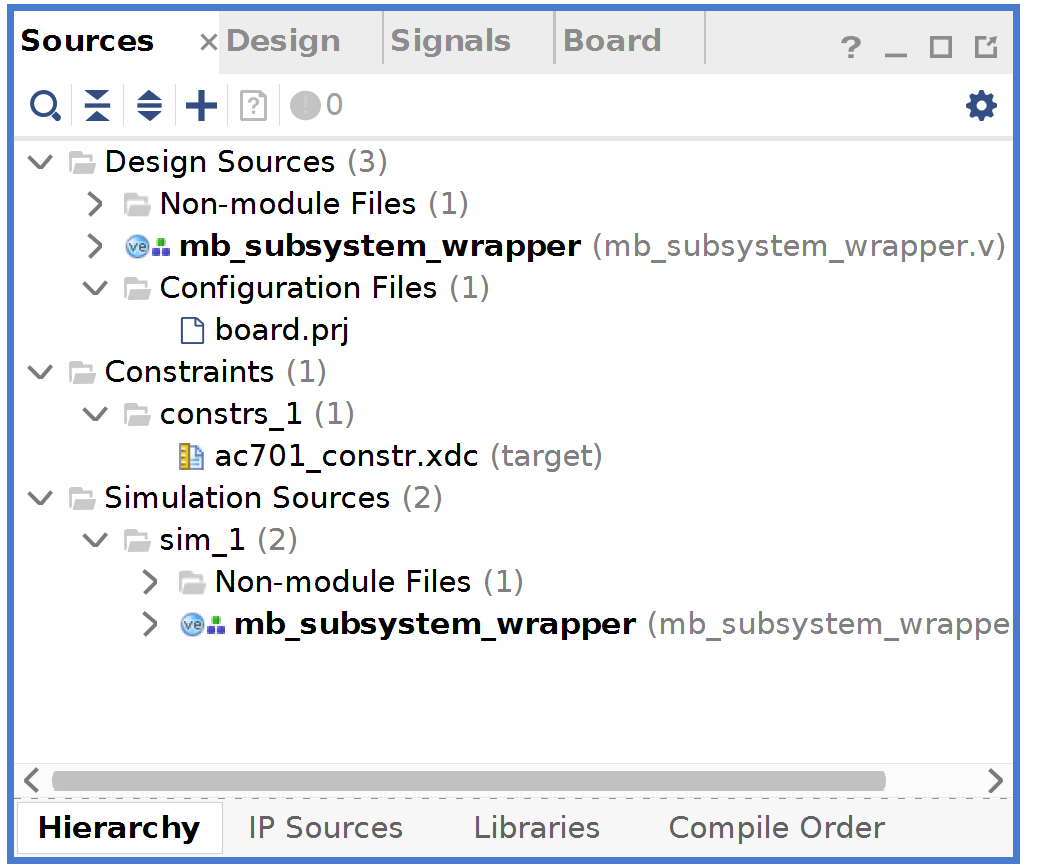
\includegraphics[scale=0.3]{constraints_tree.png}
  \captionof{figure}{Дерево исходного кода проекта}
  \label{fig:bootstrap:configuration:constraints_tree}
\end{center}

Пример \en{constraints} файла приведён на рисунке~\ref{fig:bootstrap:configuration:constraints_file}

\begin{center}
  \centering
  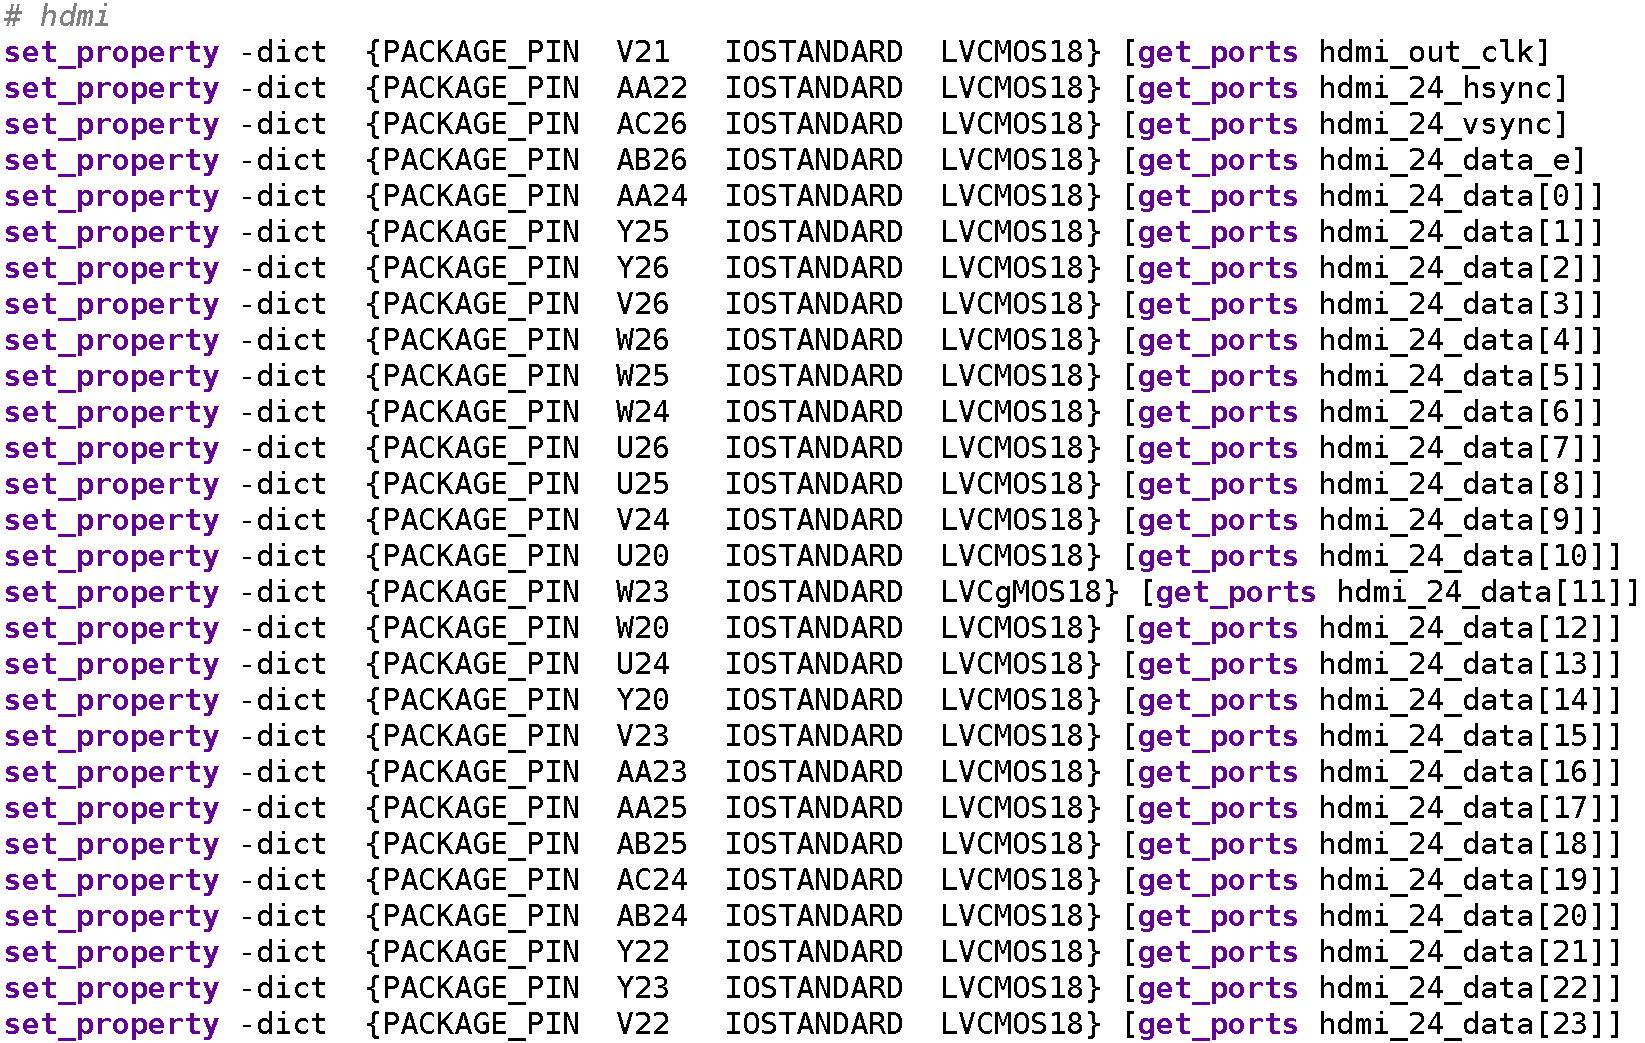
\includegraphics[scale=0.25]{constraints.png}
  \captionof{figure}{Пример \en{constraints} файла}
  \label{fig:bootstrap:configuration:constraints_file}
\end{center}

\en{Constraints} файл содержит соответствие внешних сигналов верхнего HDL модуля и
выводов микросхемы FPGA. Каждый вывод обладает уровнями допустимых напряжений, на что
следует обратить особое внимание при подключении периферии с нестандартными для FPGA
порогами. При этом только некоторые выводы могут передавать высокочастотные
тактовые сигналы, поэтому для выделения списка кандидатов на подключение из всего
множества выводов следует обратиться к технической документации микросхемы либо
предоставить выбор полуавтоматическому планировщику, работа которого должна сопровождаться
помощью со стороны пользователя.

Все необходимые изменения внешних сигналов системы могут производиться как в \en{block design},
так и в верхнем HDL модуле. При внесении изменений требуется перегенерировать модуль. Для
этого требуется открыть диалоговое меню при клике на файл на вершине иерархии, после чего выбрать пункт
\en{Create HDL Wrapper} и выбрать автоматическое обновление при изменении схемы проекта. Пример создания
верхнего модуля HDL приведено на рисунке~\ref{fig:bootstrap:configuration:hdl_wrapper}

\begin{center}
  \centering
  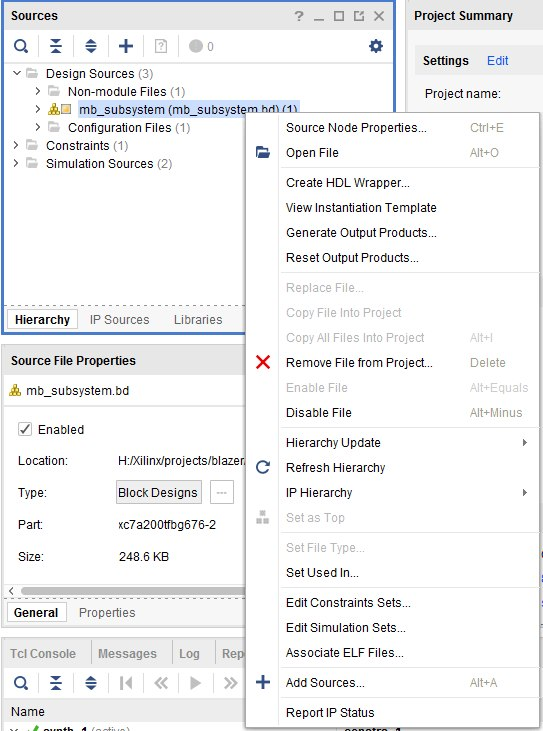
\includegraphics[scale=0.4]{hdl_wrapper.jpg}
  \captionof{figure}{Создание верхнего модуля HDL}
  \label{fig:bootstrap:configuration:hdl_wrapper}
\end{center}

После внесения изменений в проект следует этап синтезирования, реализации
синтезированного устройства на блоках микросхемы и генерация битстрима.

\subsection{Сборка проекта}
\label{sec:bootstrap:compilation}

Сборка проекта делится на несколько этапов, каждый из которых зависит от успешного
результата предыдущего.

На этапе синтеза HDL код переводится на уровень RTL (\en{Register Transfer Level}).
При наличии несинтезируемых конструкций в коде синтез прерывается с ошибкой. На этапе
синтеза присутствует возможность перезадать \en{constraints}, сменить метод синтеза и
просмотреть синтезированную схему. Пример синтезированной схемы представлен
на рисунке~\ref{fig:bootstrap:compilation:synthesis_result}

\begin{center}
  \centering
  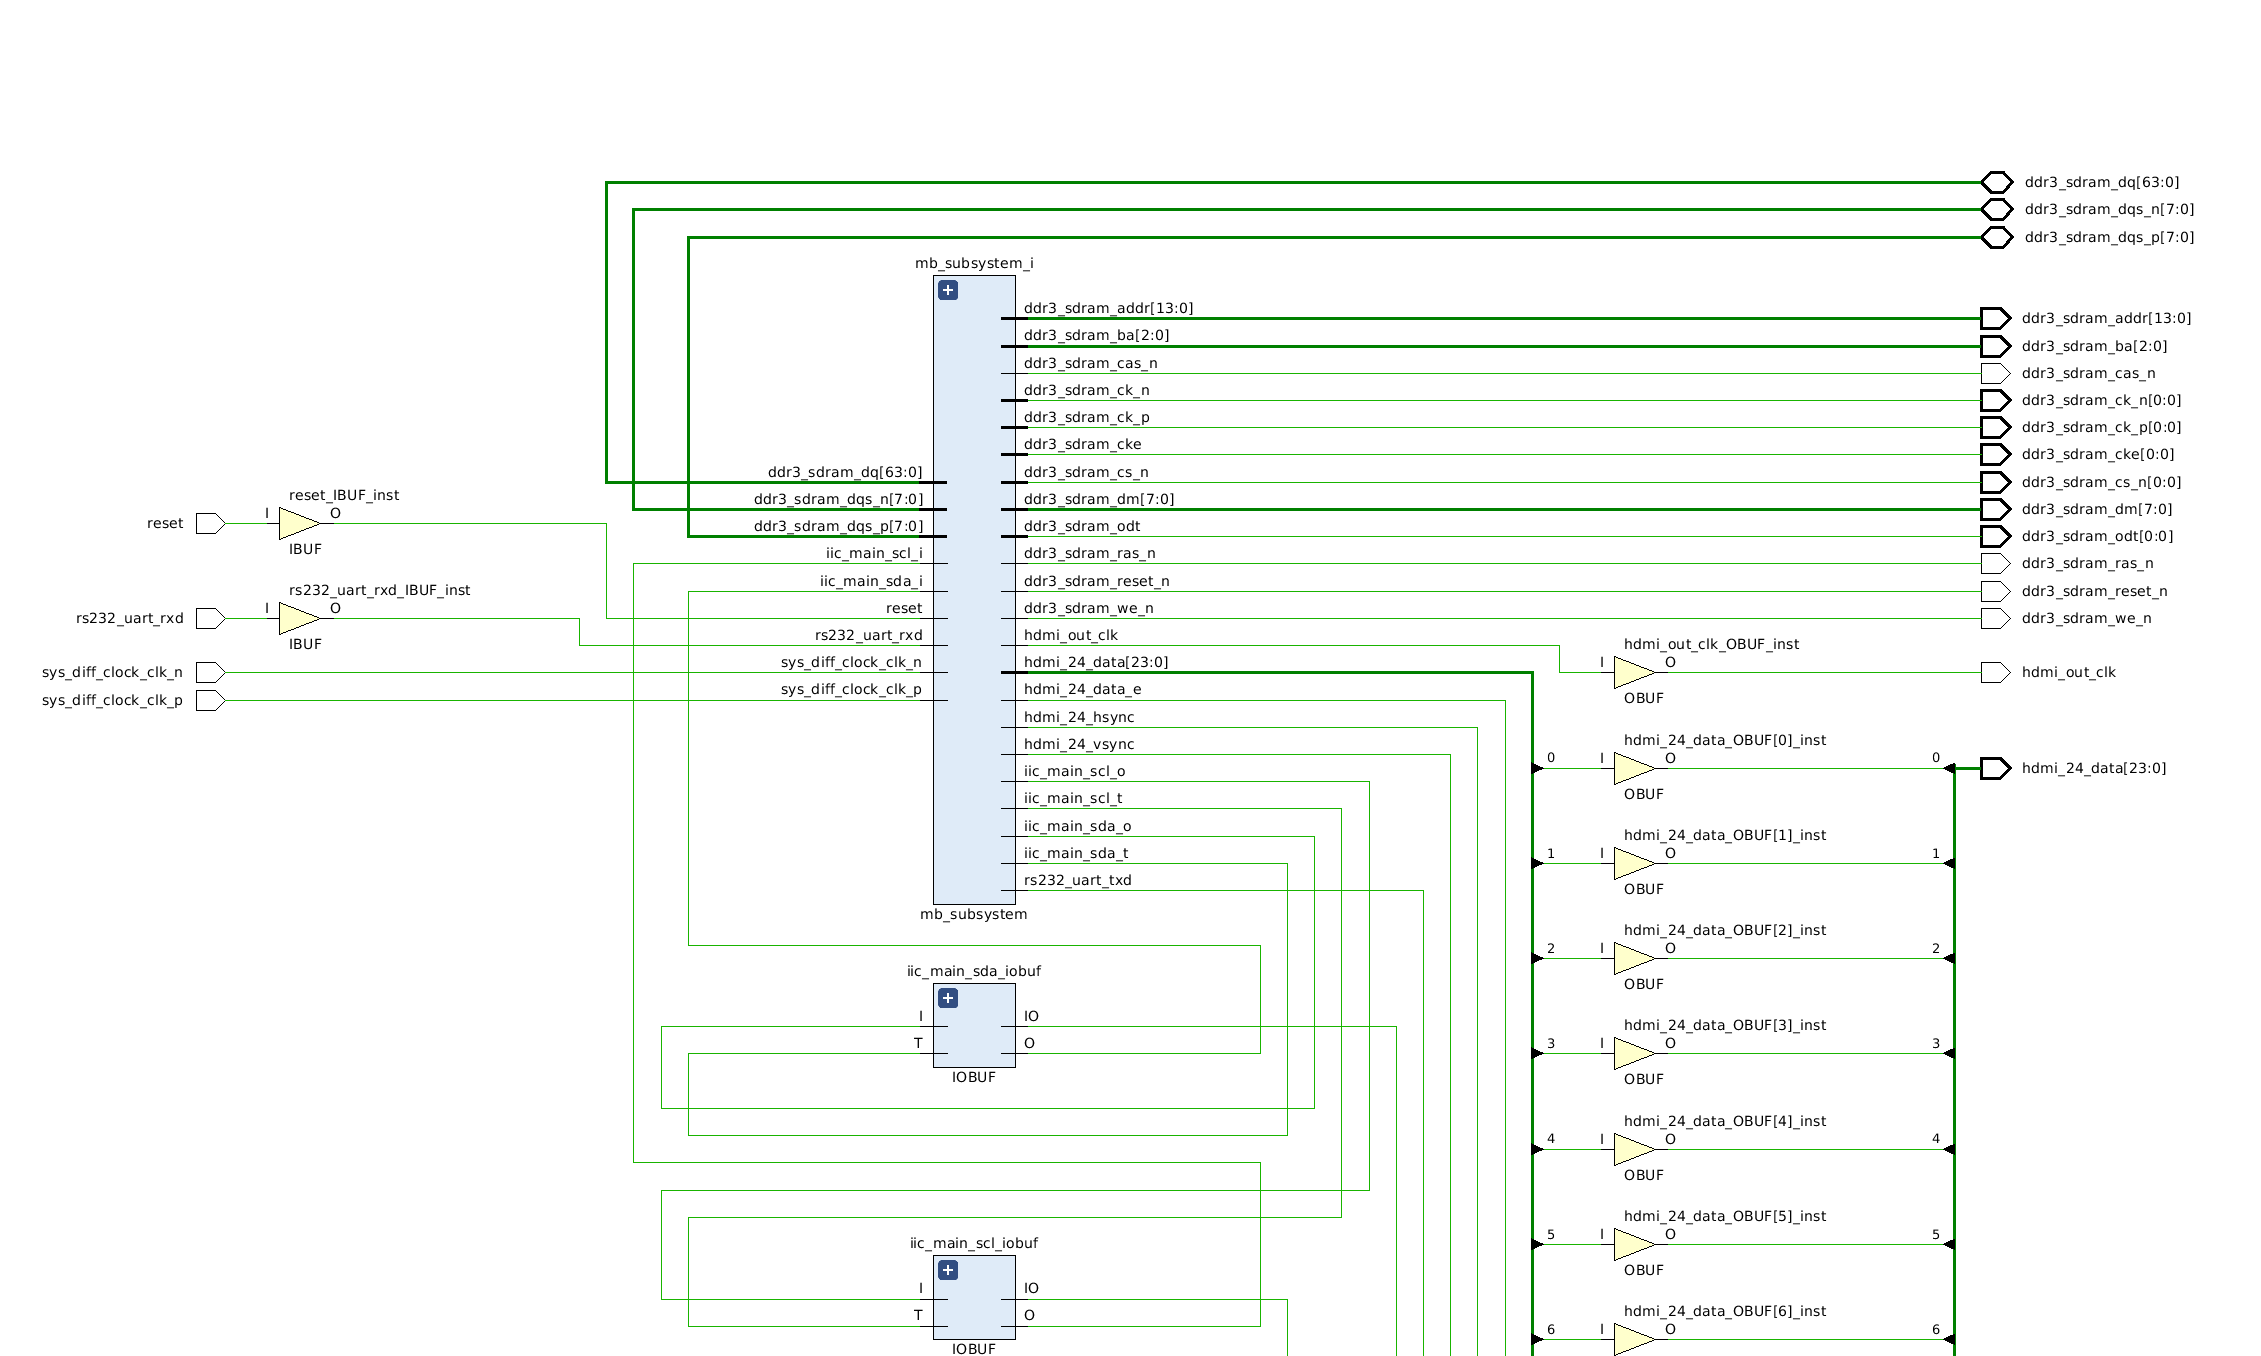
\includegraphics[scale=0.2]{synthesis_result.png}
  \captionof{figure}{Пример синтезированной схемы}
  \label{fig:bootstrap:compilation:synthesis_result}
\end{center}

Запуск синтеза производится соответствующим пунктом \en{Flow Navigator}. Блок работы с
синтезом представлен на рисунке~\ref{fig:bootstrap:compilation:synthesis_menu}

\begin{center}
  \centering
  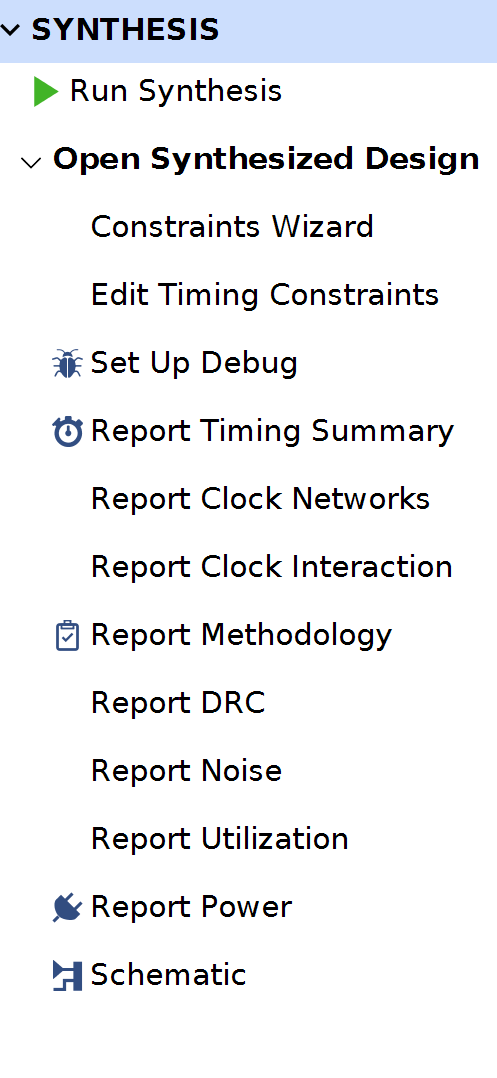
\includegraphics[scale=0.2]{synthesis_menu.png}
  \captionof{figure}{Блок работы с синтезом}
  \label{fig:bootstrap:compilation:synthesis_menu}
\end{center}

На этапе имплементации происходит реализация синтезированной схемы на логических блоках FPGA.
При этом каждому синтезированному блоку назначается КЛБ микросхемы, после назначения происходит
проводка маршрутов по трассам межсоединений. Алгоритмы имплементации занимаются поиском первого
подходящего по ограничения результата, а не лучшего среди нескольких кандидатов. Поэтому доведение
имплементации происходит путём модификации ограничений, подгоняя ограничения под различные случаи.

Пример реализации системы на ресурсах микросхемы
представлен на рисунке~\ref{fig:bootstrap:compilation:implementation_result}

\begin{center}
  \centering
  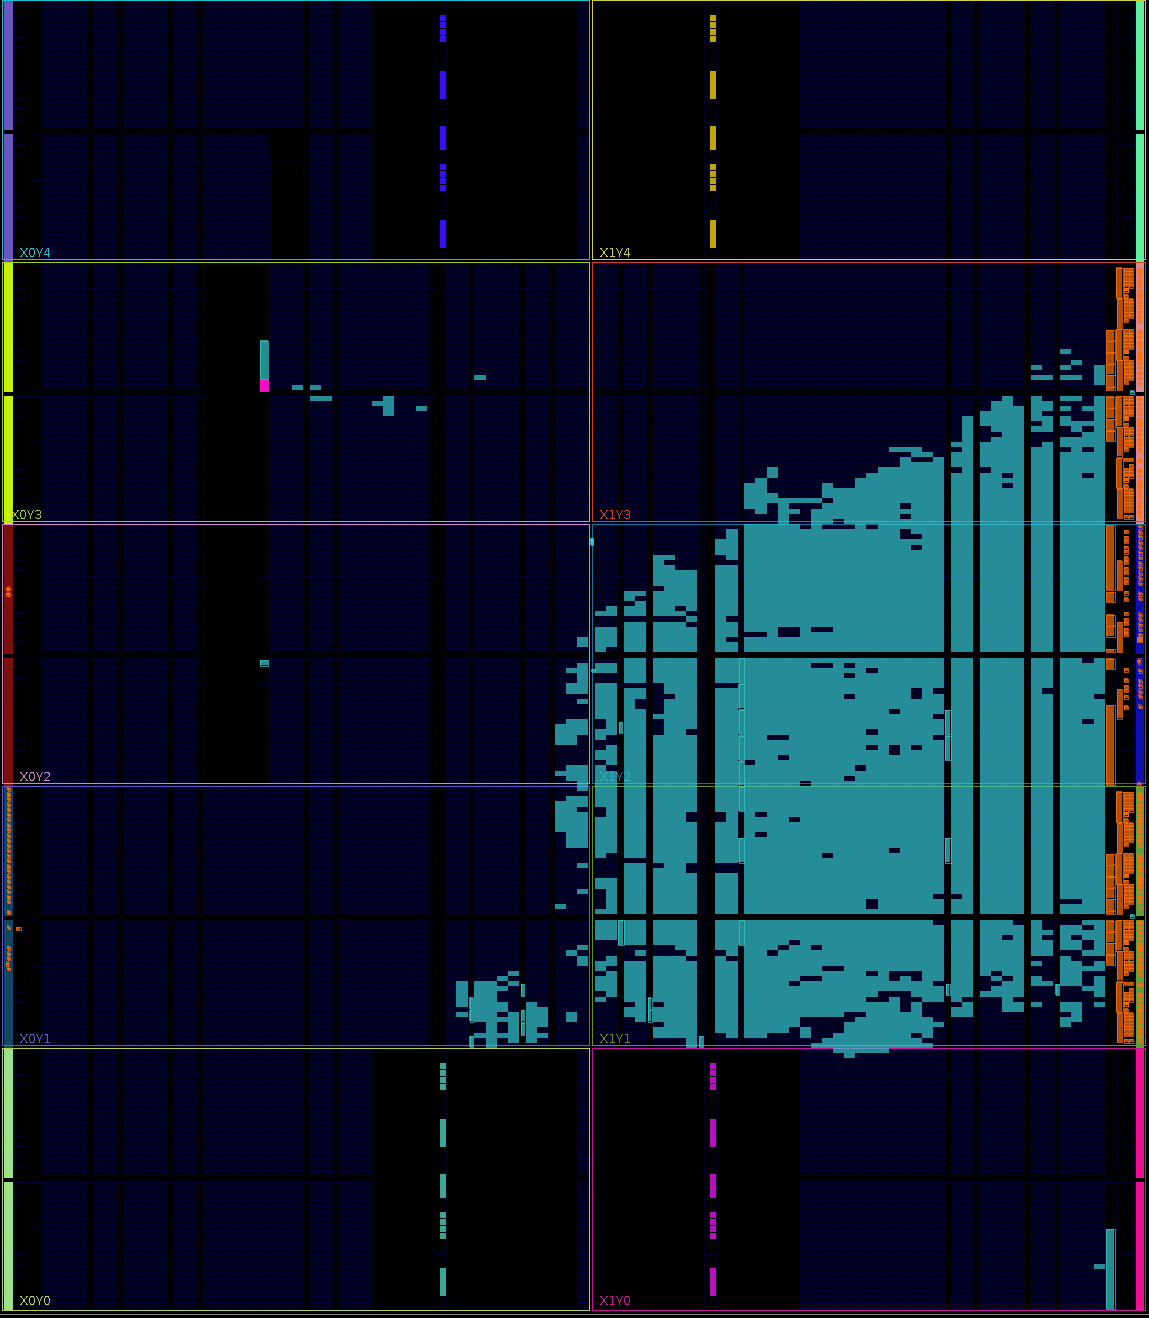
\includegraphics[scale=0.15]{implementation_result.png}
  \captionof{figure}{Результат имплементации системы}
  \label{fig:bootstrap:compilation:implementation_result}
\end{center}

Задать соответствие выводов микросхемы и выходов имплементированной схемы можно во вкладке \en{I/O Planning},
при этом стоит учесть описание назначения каждого вывода. Пример планировки выводов микросхемы
приведён на рисунке~\ref{fig:bootstrap:compilation:io_planning}

\begin{center}
  \centering
  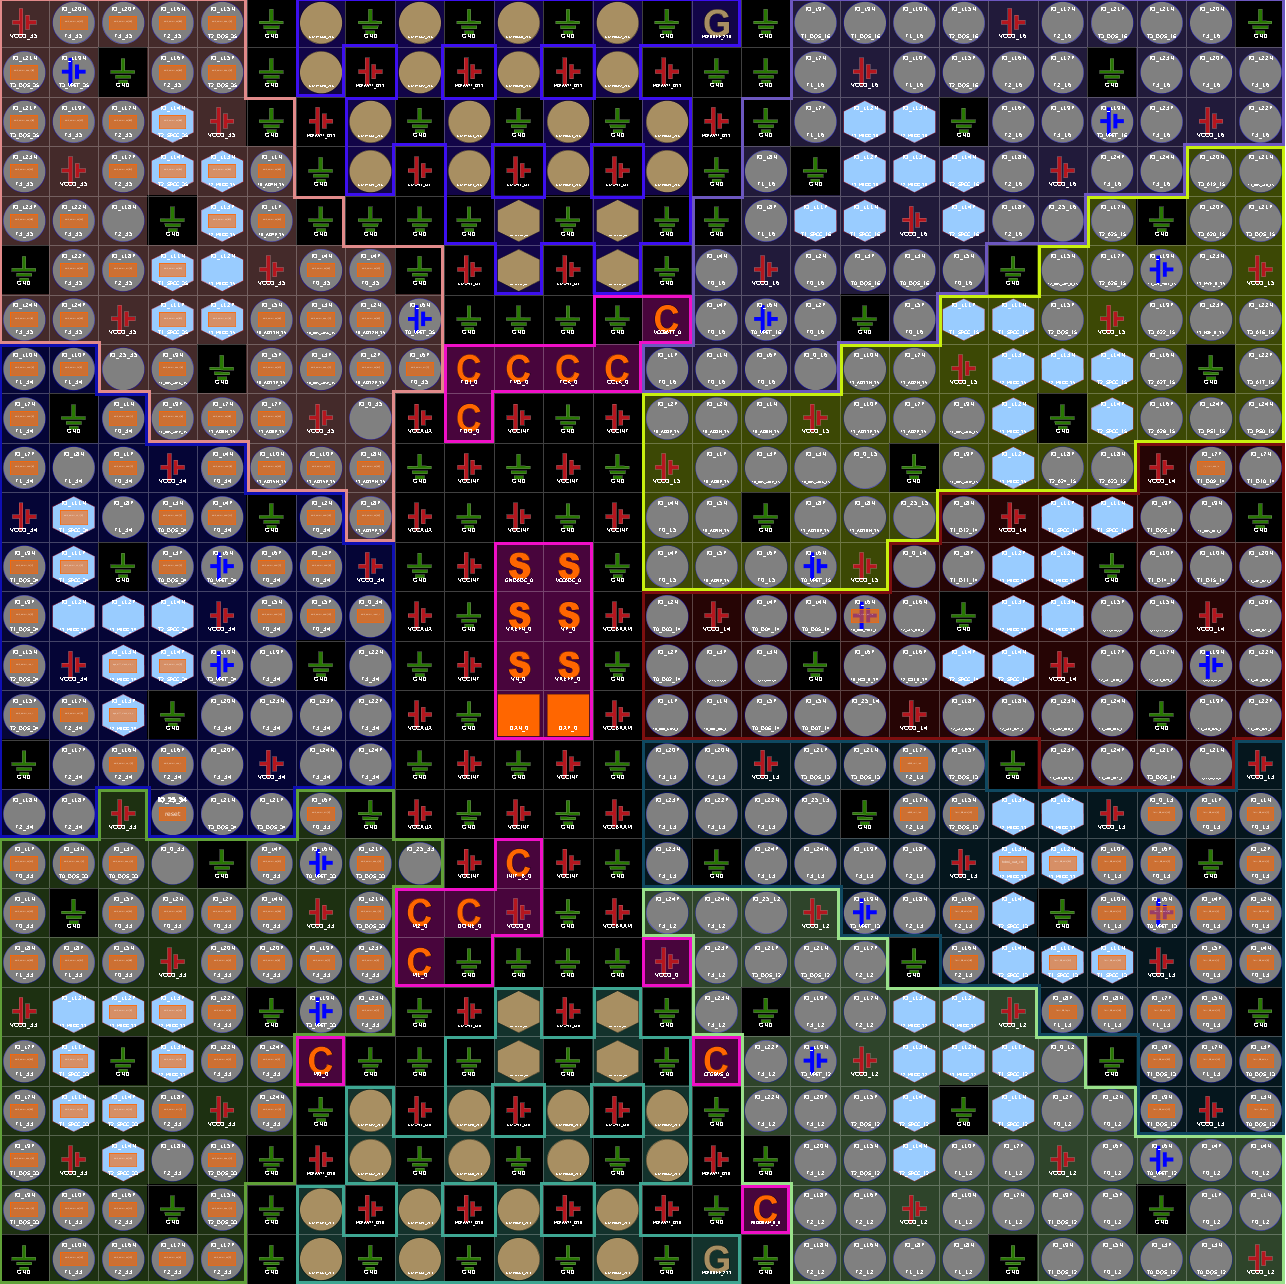
\includegraphics[scale=0.17]{io_planning.png}
  \captionof{figure}{Планировка назначения выводов микросхемы}
  \label{fig:bootstrap:compilation:io_planning}
\end{center}

Для запуска результата имплементации на микросхеме необходимо сгенерировать бистрим ---
поток битов, описывающих функциональное назначение блоков микросхемы и взаимосвязь
между ними. Процесс генерации битстрима схож с запуском синтеза.

\subsection{Запуск на отладочной плате}
\label{sec:bootstrap:board}

Далее будет описываться последовательность действий для отладочной платы
AC701. Для подготовки платы требуется выполнить следующие действия:
\begin{itemize}
  \item включить блок питания в сеть и подключить разъём к плате;
  \item подключить \en{Micro-USB} к соответствующему разъёму;
  \item подключить \en{Mini-USB} к конвертеру \en{USB to JTAG};
  \item перевести движковый переключатель питания в положение \en{On}.
\end{itemize}

После загорания на плате индикаторных светодиодов необходимо загрузить
битстрим и экспортировать аппаратную конфигурацию для последующего
применения в SDK.Экспорт аппаратной конфигурации осуществляется в
меню \en{File:Export:Export Hardware}, с выставленной опцией \en{Include Bitstream}.


После экспортирования конфигурации требуется запустить SDK из меню \en{File}.
Импорт проекта осуществляется в окне \en{Open Projects from File System} в меню \en{File}.
После успешного импорта проекта необходимо нажать пункт \en{Run Configurations} и
указать настройки согласно рисунку~\ref{fig:bootstrap:compilation:run_configuration}

\begin{center}
  \centering
  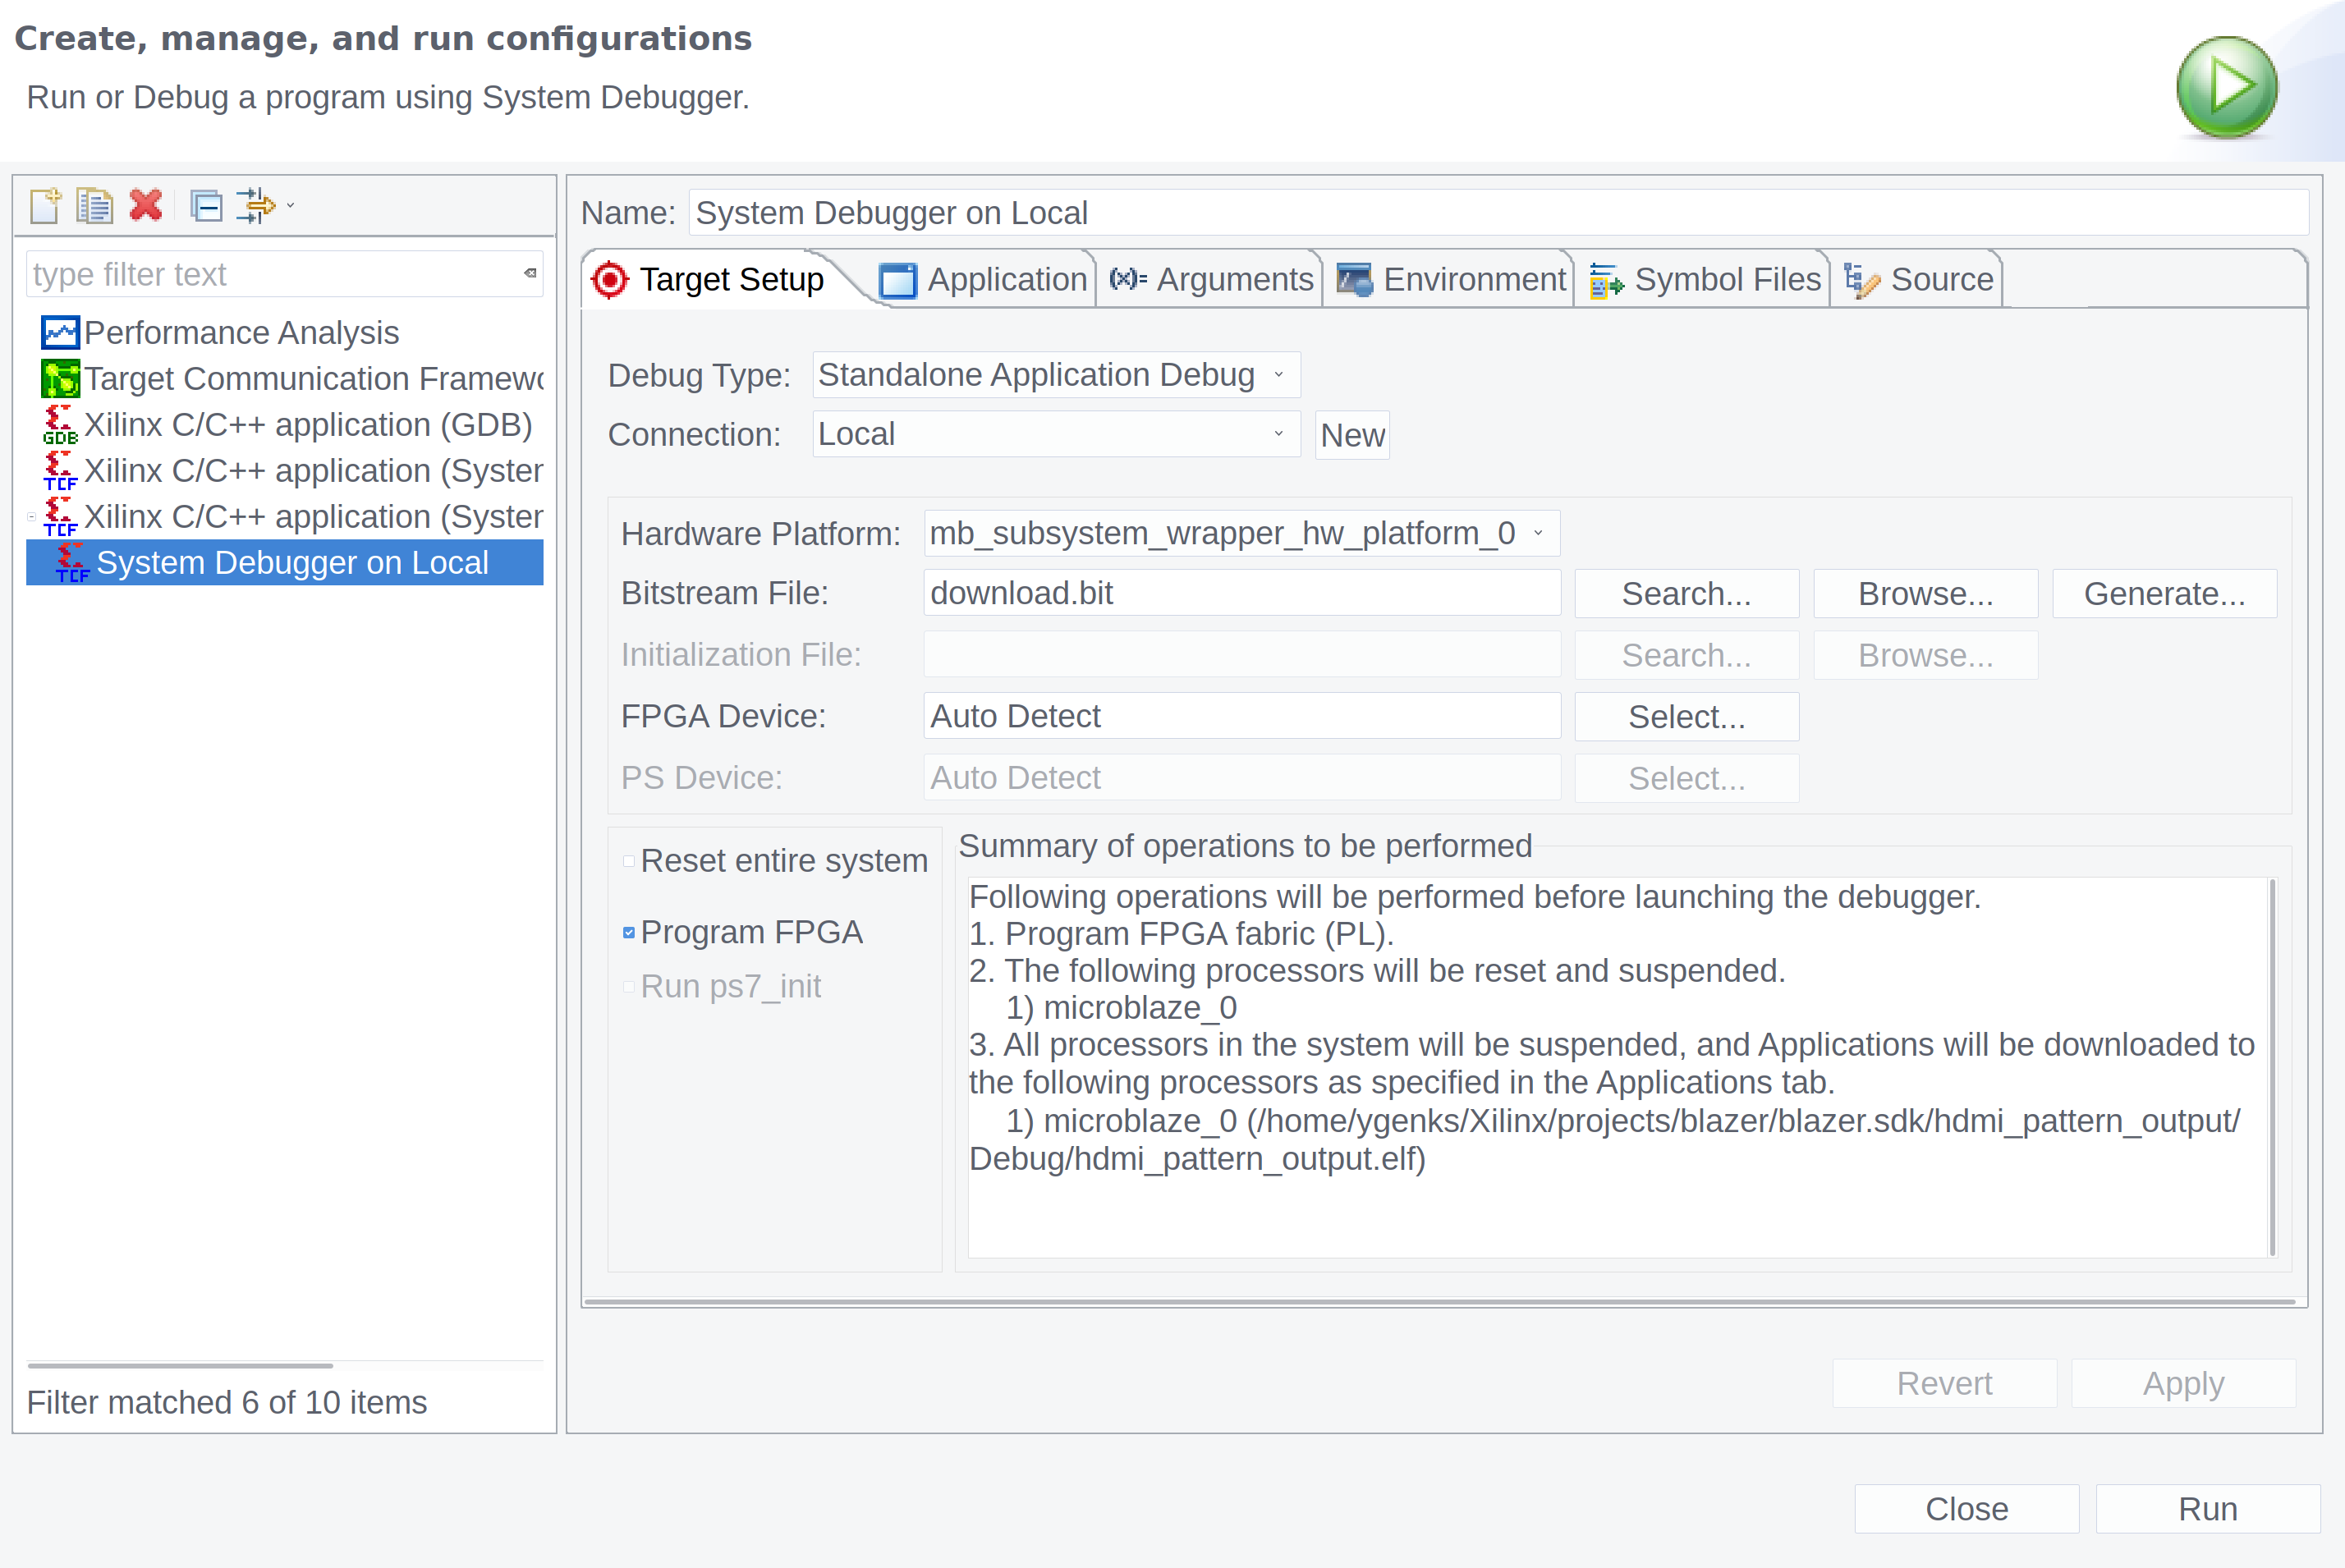
\includegraphics[scale=0.11]{run_configuration.png}
  \captionof{figure}{Конфигурация запуска}
  \label{fig:bootstrap:compilation:run_configuration}
\end{center}

Для загрузки битстрима необходимо нажать кнопку \en{Open Target} в
открытом проекте \en{Vivado}, после чего выбрать отладочную плату и начать загрузку.

После указания настроек для конфигурации запуска требуется нажать кнопку \en{Program FPGA},
указать настройки согласно рисунку~\ref{fig:bootstrap:compilation:program_fpga} и нажать
\en{Program}. При этом должны замигать индикаторы, находящиеся возле коннектора JTAG.

\begin{center}
  \centering
  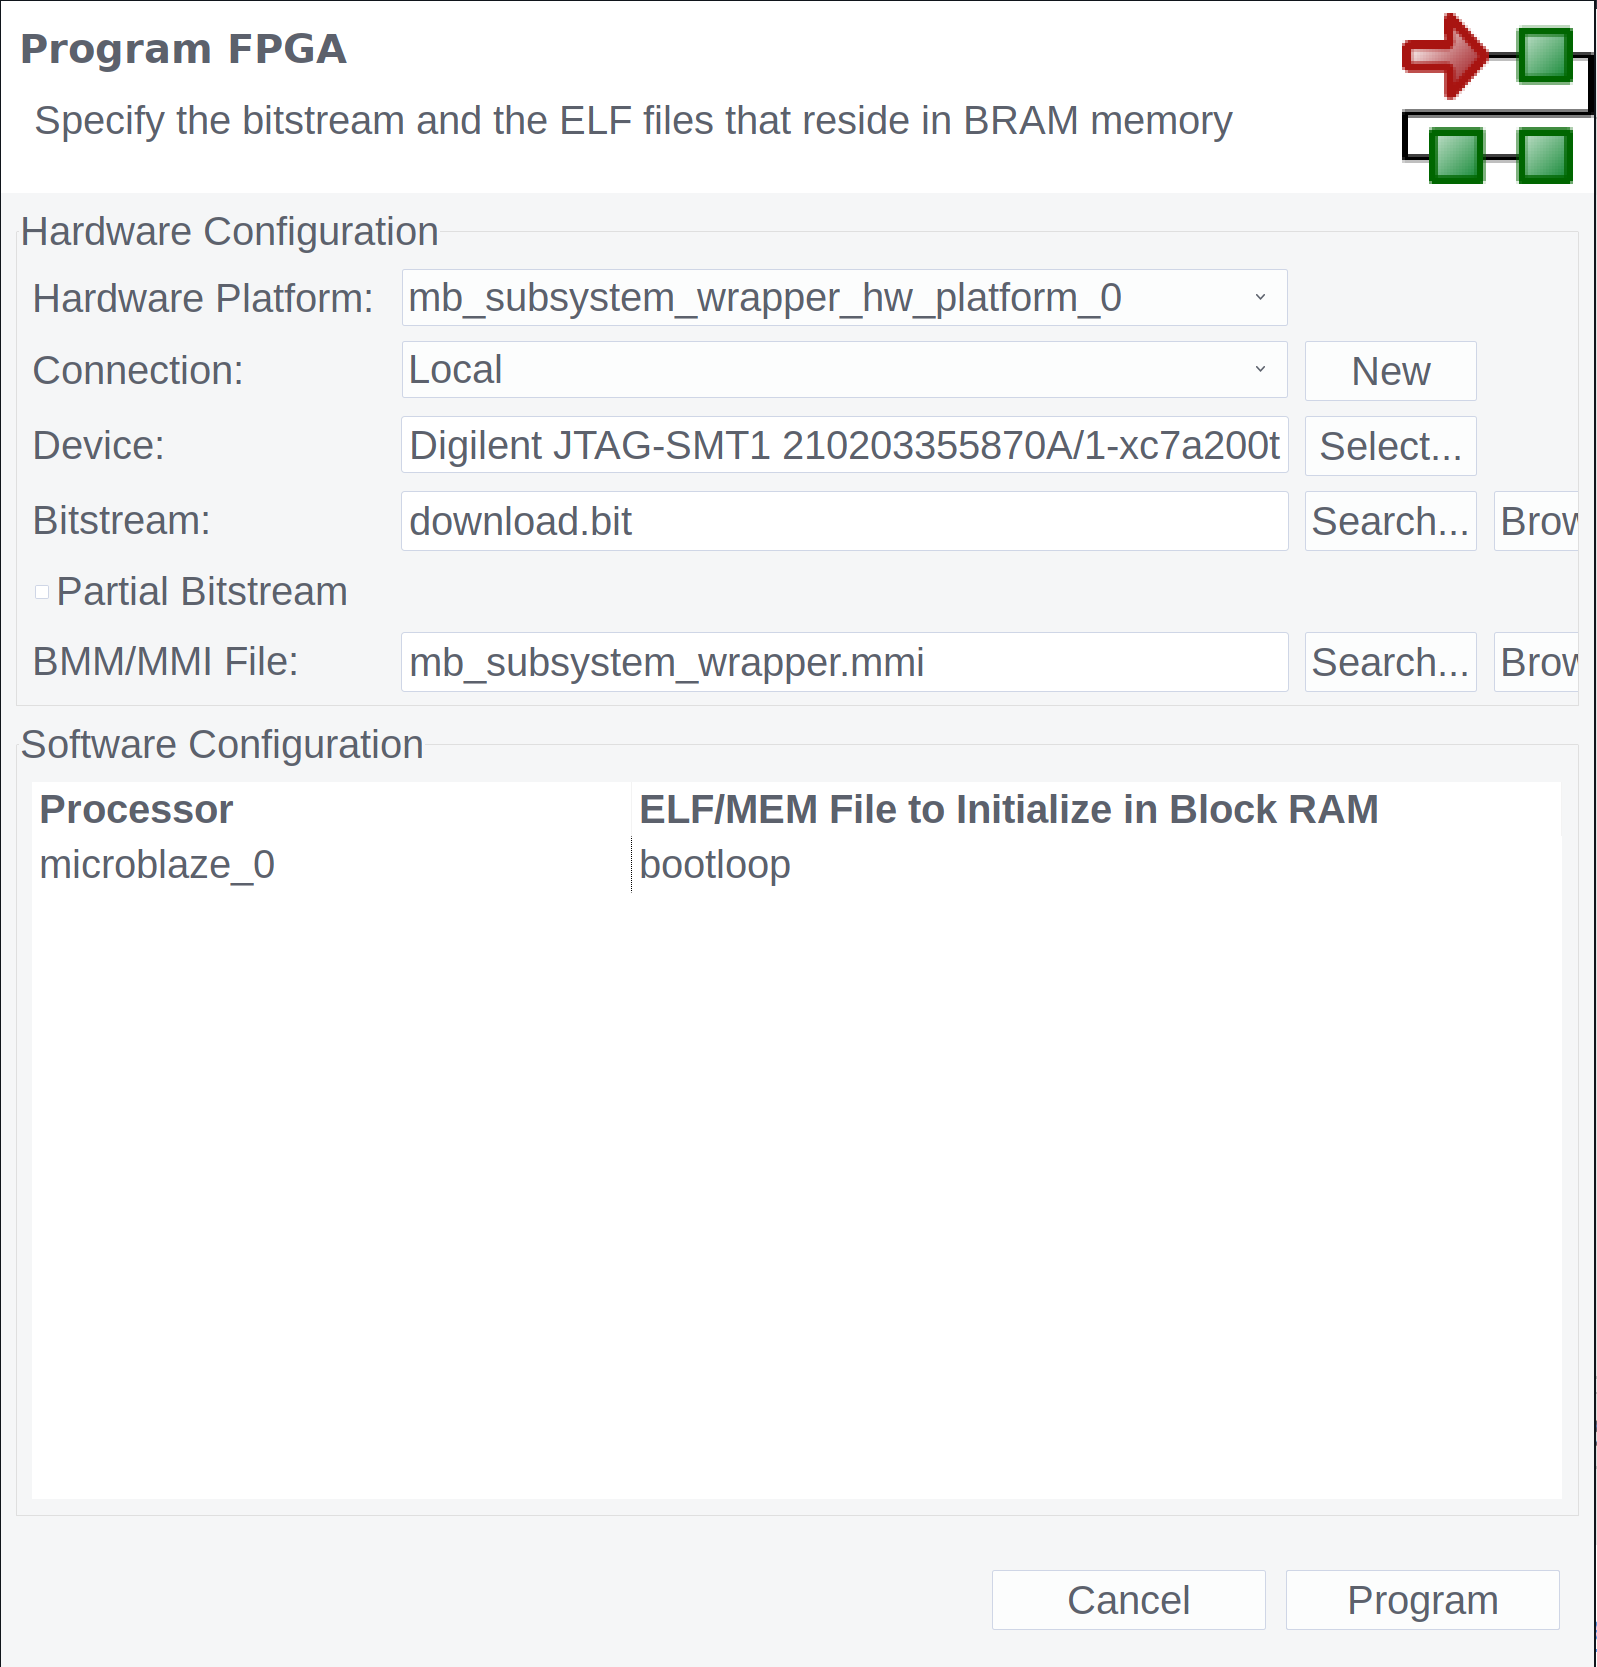
\includegraphics[scale=0.18]{program_fpga.png}
  \captionof{figure}{Загрузка битстрима в FPGA}
  \label{fig:bootstrap:compilation:program_fpga}
\end{center}

Для запуска проекта, в случае успешной загрузки битстрима, требуется нажать кнопку \en{Run} и
дождаться окончания сборки.
